\section{Evaluation}

We compare HySparse2 with HySparse~\citep{hysparse} and Hybrid SWA used in MiMo-V2 Series~\citep{xiao2026mimo}.
The overall comparison covers model performance, prefill FLOPs, and KV-cache storage.
We then conduct ablation studies on sparse selection granularity, the forced local window, and KV Bridging. 
Token-level selection targets stronger long-context accuracy in agentic scenarios without compromising efficiency, whereas the forced local window and KV Bridging target lower prefill costs while retaining model quality.

\subsection{Experimental Setup}
\label{sec:eval-setup}

\paragraph{Model configuration.}
Unless otherwise specified, experiments use 80B-A3B MoE models.
Each model has 49 Transformer layers with a hidden size of 2,048 and uses a simplified mHC variant~\citep{zhu2025hyperconnections,xie2026mhc} with the residual mixing matrix fixed to the identity. 

The models only differ in their attention designs, as summarized in Table~\ref{tab:eval-model-config}.
Full attention in every layer is the strongest reference under our evaluation. When choosing how many full-attention layers a hybrid model uses, we avoid a substantial accuracy gap from this baseline. Hybrid SWA retains nine full-attention layers, as using fewer significantly degrades accuracy. HySparse and HySparse2 each use only five full-attention layers while remaining comparable to the full-attention baseline.
Hybrid SWA and HySparse use GQA~\citep{gqa}, whereas HySparse2 uses MQA~\citep{mqa}, which yields a smaller KV cache and better token sparse attention kernel efficiency.

\begin{table}[H]
    \centering
    \small
    \setlength{\tabcolsep}{10pt}
    \begin{tabular}{lccc}
        \toprule
        \textbf{Model} & \textbf{\#Full} & \makecell{\textbf{Heads}\\\textbf{(Q/KV)}} & \makecell{\textbf{Head dim.}\\\textbf{(QK/V)}} \\
        \midrule
        Hybrid SWA & 9 & 64/4 & 192/128 \\
        HySparse & 5 & 64/4 & 192/128 \\
        HySparse2 & 5 & 64/1 & 256/256 \\
        \bottomrule
    \end{tabular}
    \caption{Configurations of the three attention designs.}
    \label{tab:eval-model-config}
\end{table}

In HySparse2, SWA layers in the self-decoder use partial rotary positional embeddings (RoPE)~\citep{rope} with 64 rotary dimensions and a base of 10,000, while full and sparse attention use NoPE.
HySparse2 therefore requires no RoPE adjustment during long-context extension.
Across the three configurations, all sparse and SWA layers use sigmoid output gates~\citep{qiu2025gated} and learnable per-head sink biases~\citep{gpt-oss}.
HySparse2 uses token-level selection with 128 forced local tokens and 1,024 global tokens.
HySparse selects 1,024 global tokens in 64-token blocks and combines sparse attention with a separate 128-token SWA branch through gated fusion.
Hybrid SWA uses a sliding window of 128 tokens.

\paragraph{Training.}
We pretrain the 80B-A3B models on approximately 500B tokens at a context length of 32k.
A light post-training stage adds approximately 100B tokens, introduces agentic data into the training mixture, and extends the context length to 256k.
The three models share the same data mixture and training schedule within each stage.
We use the Muon optimizer~\citep{jordan2024muon} with a WSD schedule and peak learning rates of $10^{-3}$ for pretraining and $5\times10^{-5}$ for post-training.
We report both pretraining and post-training results for overall comparisons, and only pretraining results for ablations.

\paragraph{Evaluation.}



The pretraining evaluation covers knowledge (MMLU, MMLU-Redux, MMLU-Pro, C-Eval, CMMLU, TriviaQA)~\citep{mmlu,gema2024we,wang2024mmlu,huang2023c,li2023cmmlu,joshi2017triviaqa}, reasoning (BBH, MATH, DROP, GSM8K, ARC-C, HellaSwag, WinoGrande)~\citep{suzgun2022challenging,hendrycks2021measuring,dua2019drop,gsm8k,arcc,zellers2019hellaswag,sakaguchi2021winogrande}, code (HumanEval+, MBPP+, Repo Code PPL)~\citep{humaneval,mbpp,liu2023your}, and long-context tasks (RULER, NoLiMa)~\citep{ruler,modarressi2025nolima}, as listed in Table~\ref{tab:v2-v1-pretrain}.
Repo Code PPL is an internal benchmark that reports byte perplexity over long code repositories with cross-file dependencies, and therefore also probes long-context modeling ability.

After light post-training, we focus on multi-turn retrieval and long-context likelihood on agent trajectories.
AgentPPL is an internal benchmark built from multi-turn agent trajectories that measures byte perplexity on the reasoning, tool-call, and response segments of 1,000 trajectories.
LongPPL~\citep{fang2024longppl} measures perplexity on selected tokens that depend on long-range context, using 349 examples from agent trajectories and long-context tasks.
MRCR-v2~\citep{vodrahalli2024michelangelo} measures multi-round retrieval with two, four, or eight needles.
RULER-v2~\citep{ruler_v2_2025} covers 12 retrieval and question-answering subtasks. GraphWalks~\citep{openai2025gpt41} evaluates multi-hop graph traversal.

\subsection{Overall Comparison}
\label{sec:v2-v1}

\paragraph{Pretraining results.}

\begin{table}[t]
    \centering
    \small
    \setlength{\tabcolsep}{10pt}
    \begin{tabular}{lrrr}
        \toprule
        \textbf{Task} & \textbf{Hybrid SWA} & \textbf{HySparse} & \textbf{HySparse2} \\
        \midrule
        \multicolumn{4}{l}{\textit{Knowledge}} \\
        MMLU & 61.48 & \textbf{64.48} & 63.92 \\
        MMLU-Redux & 63.96 & \textbf{68.44} & 67.50 \\
        C-Eval & 65.08 & 67.09 & \textbf{67.90} \\
        CMMLU & 67.41 & \textbf{69.97} & 69.90 \\
        TriviaQA & 60.59 & \textbf{60.67} & 59.67 \\
        \midrule
        \multicolumn{4}{l}{\textit{Reasoning}} \\
        BBH & 60.14 & 61.93 & \textbf{64.29} \\
        MMLU-Pro & 36.12 & 35.74 & \textbf{37.56} \\
        MATH & \textbf{36.18} & 36.14 & 34.32 \\
        DROP & 60.90 & \textbf{63.78} & 58.99 \\
        GSM8K & \textbf{64.44} & 64.14 & 61.94 \\
        ARC-C & 75.51 & \textbf{79.18} & 77.82 \\
        HellaSwag & 79.38 & 79.19 & \textbf{79.54} \\
        WinoGrande & 73.72 & \textbf{74.19} & 71.82 \\
        \midrule
        \multicolumn{4}{l}{\textit{Code}} \\
        HumanEval+ & \textbf{35.98} & 34.76 & 34.15 \\
        MBPP+ & \textbf{55.56} & 52.65 & 52.65 \\
        Repo Code PPL $\downarrow$ & 1.1578 & 1.1588 & \textbf{1.1570} \\
        \midrule
        \multicolumn{4}{l}{\textit{Long context}} \\
        RULER & 88.71 & 84.89 & \textbf{90.77} \\
        NoLiMa & 30.13 & 40.27 & \textbf{49.76} \\
        \bottomrule
    \end{tabular}
    \caption{Pretraining performance of the 80B-A3B models. HySparse2 improves long-context performance while remaining broadly comparable to both baselines on general capabilities.}
    \label{tab:v2-v1-pretrain}
\end{table}


Table~\ref{tab:v2-v1-pretrain} shows that HySparse2 remains broadly comparable to both baselines on general capabilities, while its clearest gains are in long-context modeling. 
HySparse2 achieves the highest RULER and NoLiMa scores, improving over HySparse by 5.88 and 9.49 points, respectively. It also has the lowest Repo Code PPL at 1.1570, a small improvement over 1.1588 for HySparse and 1.1578 for Hybrid SWA. Individual general-purpose results show a mixed picture. HySparse2 is stronger on BBH and MMLU-Pro, while HySparse retains an advantage on DROP.




\paragraph{Agentic and long-context results.}

We next compare the models after the same light post-training stage of approximately 100B tokens.
We evaluate retrieval with MRCR-v2 and RULER-v2 and long-context likelihood with AgentPPL and LongPPL. Retrieval averages weight the reported context lengths equally, and perplexity curves group examples by context length.

Figure~\ref{fig:v2-v1-posttrain} shows that HySparse2 leads both baselines on all four metrics at every evaluated length.
The largest gains are in retrieval.
Relative to HySparse, its mean MRCR-v2 and RULER-v2 scores increase by 11.30 and 19.81 points, while the corresponding gains over Hybrid SWA are 6.44 and 18.65 points.
The advantage remains large at 256k, where HySparse2 reaches 58.45 on RULER-v2, compared with 32.61 for HySparse and 35.74 for Hybrid SWA. 
HySparse2 also achieves lower AgentPPL and LongPPL throughout the evaluated range, showing that its retrieval gains are accompanied by better likelihood on long agent trajectories and context-dependent tokens.
AgentPPL increases with context length, whereas LongPPL decreases.
This contrast reflects opposite effects of additional context: longer contexts expose more relevant information for LongPPL's key tokens, but also introduce more intervening turns and tool outputs that make the relevant evidence harder to retrieve in multi-turn agent trajectories.



\begin{figure}[H]
    \centering
    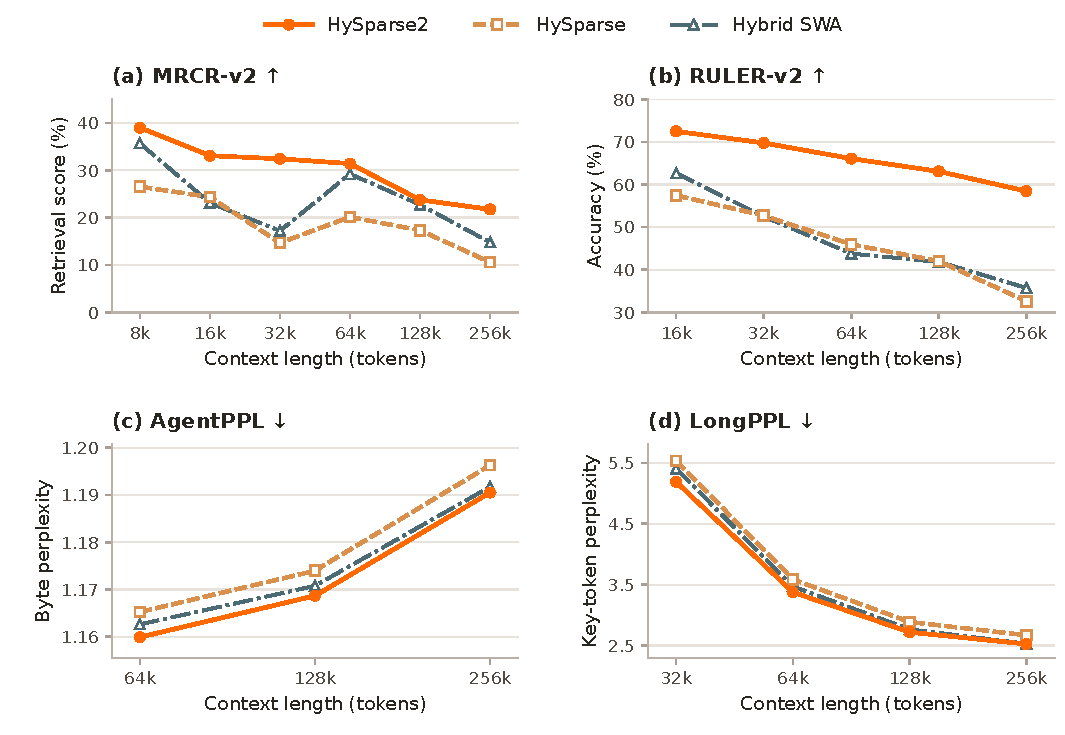
\includegraphics[width=\linewidth]{figures/v2_vs_v1_posttrain.pdf}
    \caption{Long-context performance after a light post-training stage. HySparse2 achieves higher retrieval scores and lower perplexity than both baselines across all evaluated context lengths.}
    \label{fig:v2-v1-posttrain}
\end{figure}


\paragraph{Prefill computation and KV-cache storage.}


We compare the prefill FLOPs and KV-cache size of HySparse2, HySparse, and Hybrid SWA, under the 80B-A3B configuration across context lengths from 1k to 1M tokens with FP8 KV-cache storage.


Figure~\ref{fig:prefill-costs} shows that HySparse2 requires less prefill computation and KV-cache storage than HySparse and Hybrid SWA.
At 1M tokens, HySparse2 reduces prefill FLOPs by $2.92\times$ relative to HySparse and $5.02\times$ relative to Hybrid SWA.
The KV cache of HySparse2 occupies only 2.69\,GB, compared with 6.72\,GB for HySparse and 12.09\,GB for Hybrid SWA.


\begin{figure}[h]
    \centering
    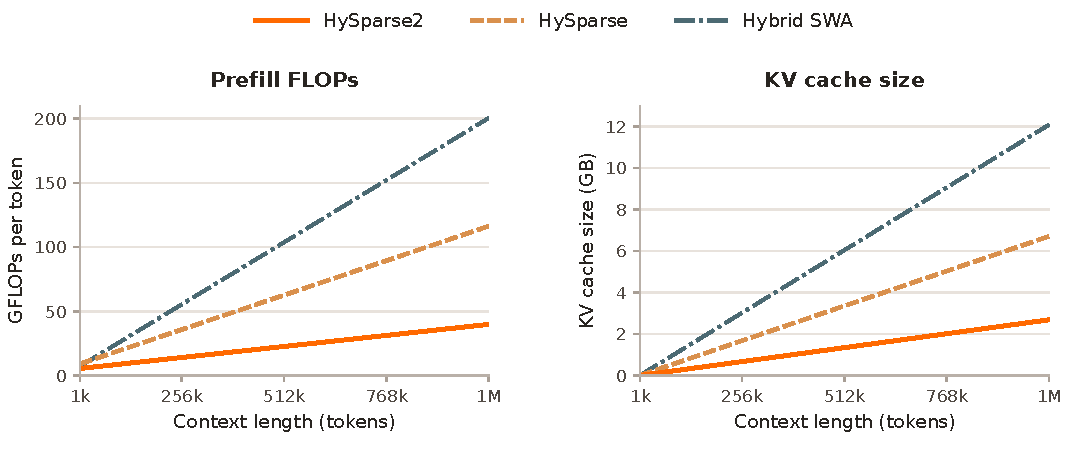
\includegraphics[width=\linewidth]{figures/prefill_costs.pdf}
    \caption{Prefill computation and KV-cache storage for the 80B-A3B models. HySparse2 reduces both costs relative to HySparse and Hybrid SWA.}
    \label{fig:prefill-costs}
\end{figure}

\subsection{Ablation 1: Token-Level versus Block-Level Sparsity}
\label{sec:token-block-ablation}

We compare block-level selection with token-level selection.
Block-level selection uses a block size of 64.
Both variants use the same backbone layout, select 1,024 global tokens, and retain a separate 128-token local window.

\begin{table}[H]
    \centering
    \small
    \setlength{\tabcolsep}{10pt}
    \begin{tabular}{lrr}
        \toprule
        \textbf{Task} & \textbf{Block} & \textbf{Token} \\
        \midrule
        \multicolumn{3}{l}{\textit{Pretraining}} \\
        BBH & \textbf{61.93} & 60.70 \\
        MMLU-Pro & 35.74 & \textbf{36.97} \\
        NoLiMa & \textbf{40.27} & 38.43 \\
        \midrule
        \multicolumn{3}{l}{\textit{Long context ($\leq$32k)}} \\
        RULER-v2 & 49.56 & \textbf{56.13} \\
        MRCR-v2 (2-needle) & 12.94 & \textbf{21.08} \\
        GraphWalks & 29.38 & \textbf{34.92} \\
        \bottomrule
    \end{tabular}
    \caption{Token-level versus block-level sparse selection after pretraining. Token-level selection improves long-context retrieval and graph reasoning under the same attention budget.}
    \label{tab:token-block-ablation}
\end{table}

Table~\ref{tab:token-block-ablation} shows clear gains for token-level selection on long-context retrieval and graph reasoning under the same attention budget.
It improves RULER-v2 by 6.57 points, two-needle MRCR-v2 by 8.14 points, and GraphWalks by 5.55 points.
These gains are present within the 32k training context.

Agent trajectories repeatedly interleave reasoning, tool calls, and returned observations.
The information needed for a response can be spread across several turns, along with role delimiters and other special tokens that identify the relevant boundaries.
Under a fixed attention budget, selecting a block to retain one such token also spends capacity on its neighbors.
Token-level selection can allocate that budget to individual positions across the context.
The retrieval and graph-reasoning gains are consistent with this explanation.

\subsection{Ablation 2: Local Window in Sparse Layers}
\label{sec:swa-ablation}

We compare three ways to handle local context inside sparse layers: a separate gated 128-token SWA branch (\textbf{Gated SWA}), removing the separate SWA branch (\textbf{No SWA}), and forcing the most recent 128 tokens into the sparse selection (\textbf{Forced SWA}).
All three share the same model backbone, KV Bridging, and hybrid SWA self-decoder. They differ only in how the cross-decoder's sparse attention handles local context.
We evaluate pretraining results within their 32k training context.

\begin{table}[H]
    \centering
    \small
    \setlength{\tabcolsep}{10pt}
    \begin{tabular}{lrrr}
        \toprule
        \textbf{Task} & \textbf{Gated SWA} & \textbf{No SWA} & \textbf{Forced SWA} \\
        \midrule
        \multicolumn{4}{l}{\textit{Reasoning}} \\
        BBH & 62.23 & 60.11 & \textbf{62.25} \\
        MMLU-Pro & \textbf{39.15} & 37.19 & 38.12 \\
        MATH & \textbf{35.82} & 33.82 & 33.38 \\
        DROP & \textbf{60.06} & 58.94 & 56.85 \\
        GSM8K & \textbf{64.52} & 60.35 & 59.44 \\
        ARC-C & \textbf{81.06} & 79.01 & 78.41 \\
        HellaSwag & \textbf{79.85} & 78.23 & 78.42 \\
        WinoGrande & 73.09 & \textbf{73.95} & 72.85 \\
        \midrule
        \multicolumn{4}{l}{\textit{Long context ($\leq$32k)}} \\
        NoLiMa & 37.62 & \textbf{38.37} & 36.16 \\
        RULER & 88.19 & 84.55 & \textbf{89.84} \\
        RULER-v2 & 53.66 & 54.62 & \textbf{55.98} \\
        MRCR-v2 & \textbf{27.66} & 20.73 & 22.67 \\
        GraphWalks & 35.39 & 36.48 & \textbf{37.13} \\
        LongPPL $\downarrow$ & \textbf{6.8807} & 7.1307 & 6.9838 \\
        \bottomrule
    \end{tabular}
    \caption{Local-attention ablation in sparse layers. Forced SWA remains competitive with Gated SWA.}
    \label{tab:swa-ablation}
\end{table}


Table~\ref{tab:swa-ablation} shows that local information is necessary for sparse attention. Removing the local branch (No SWA) generally degrades model performance, while Forced SWA remains competitive with Gated SWA on several tasks.
Forced SWA achieves the best RULER, RULER-v2, and GraphWalks scores. Compared with Gated SWA, Forced SWA is 5.08 points lower on GSM8K and 4.99 points lower on MRCR-v2, while LongPPL is 1.50\% higher.
We consider this an acceptable trade-off, as Forced SWA avoids additional projection parameters and requires no local KV cache, thereby making early-exit prefill feasible.

\subsection{Ablation 3: KV Bridging}
\label{sec:kv-mirror-ablation}

\paragraph{With and without KV Bridging.}

KV Bridging is designed primarily to accelerate prefill while preserving model quality. To test whether this design scales, we train 290B-A8B models on approximately 1.8T tokens at a 32k context length, with and without KV Bridging.


\begin{table}[H]
    \centering
    \small
    \setlength{\tabcolsep}{12pt}
    \begin{tabular}{lrr}
        \toprule
        \textbf{Task} & \textbf{w/o bridging} & \textbf{w/ bridging} \\
        \midrule
        MMLU & 72.68 & \textbf{72.80} \\
        TriviaQA & 73.32 & \textbf{74.10} \\
        BBH & \textbf{70.65} & 69.57 \\
        DROP & \textbf{71.37} & 68.17 \\
        GSM8K & \textbf{77.63} & 76.65 \\
        Repo Code PPL $\downarrow$ & \textbf{1.1351} & 1.1353 \\
        RULER & \textbf{96.32} & 96.01 \\
        LongPPL $\downarrow$ & 3.6053 & \textbf{3.4202} \\
        \bottomrule
    \end{tabular}
    \caption{KV Bridging ablation at the 290B-A8B scale. Models with and without KV Bridging achieve broadly comparable quality.}
    \label{tab:kv-mirror-results}
\end{table}

Table~\ref{tab:kv-mirror-results} shows that KV Bridging preserves quality comparable to the baseline without it. MMLU and TriviaQA improve slightly, RULER changes by only 0.31 points, and Repo Code PPL is nearly unchanged. LongPPL improves from 3.6053 to 3.4202. BBH and GSM8K decrease by about one point, and DROP falls from 71.37 to 68.17.

\paragraph{KV Bridging versus KV Mirror.}
For the connection scheme, we compare KV Bridging with KV Mirror~\citep{liu2026hidden} on 80B-A3B models that share the same hybrid backbone and pretraining recipe.
KV Mirror uses U-shaped connections that pair early and late layers in reverse order, $1\!\rightarrow\!n$, $2\!\rightarrow\!n-1$, and so on, whereas KV Bridging connects only the full-attention layers in the self-decoder and the cross-decoder.
Both styles form the target KV representations by re-projecting source hidden states.


\begin{figure}[H]
    \centering
    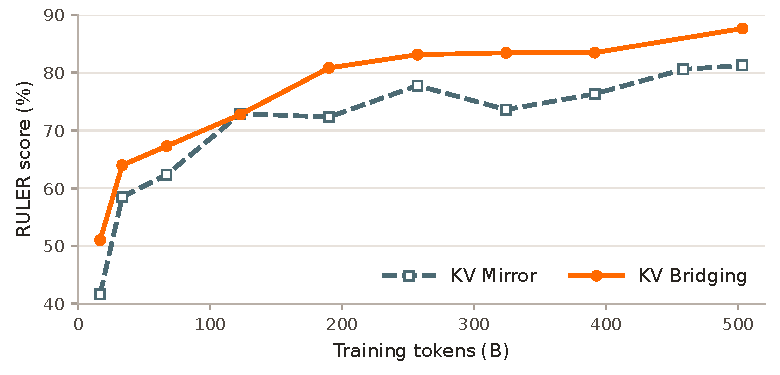
\includegraphics[width=0.8\linewidth]{figures/kv_mirror_connections.pdf}
    \caption{KV Bridging versus KV Mirror during pretraining. KV Bridging achieves higher RULER scores.}
    \label{fig:kv-mirror-connections}
\end{figure}

Figure~\ref{fig:kv-mirror-connections} shows that KV Bridging is stronger for most of training and finishes at 87.65, compared with 81.28 for KV Mirror.
We hypothesize that full-layer states are better sources because full attention backpropagates through scores across the entire visible context, while SWA restricts these direct connections to a local window.
This denser supervision produces representations that retain more global information for projection.

